\section{函数的线性运算}
\label{sec:fvec-linear-operations}

两条温度曲线可以取平均，一个信号可以整体放大一倍，一个近似函数减去目标函数得到误差函数。这些操作都作用于整个函数，结果仍是一个函数。它们遵守的规则与向量运算完全相同，原因就在于函数可以看成“每个输入占一个分量”的向量。

全章固定标量域$\mathbb K$，它是实数域$\mathbb R$或复数域$\mathbb C$。需要区分时，我们写明“实函数空间”或“复函数空间”；不写明时，结论对两种情形都成立。函数空间的元素是整个函数，按习惯用普通字母$f,g,h$或$x,y$表示，不用粗体。

\paragraph{逐点加法与数乘}
先做一个有限的计算。在$[0,1]$上取$f(x)=x^2$与$g(x)=1-x$，在四个等距点$x_1=0$、$x_2=\tfrac13$、$x_3=\tfrac23$、$x_4=1$处读出取值。每个函数由此变成一个四维向量：
\[
 \begin{aligned}
 [f(x_1),f(x_2),f(x_3),f(x_4)]&=[0,\tfrac19,\tfrac49,1],\\
 [g(x_1),g(x_2),g(x_3),g(x_4)]&=[1,\tfrac23,\tfrac13,0].
 \end{aligned}
\]
把这两个向量逐分量相加，得到
\[
 [1,\tfrac79,\tfrac79,1].
\]

函数$h(x)=x^2-x+1$在这四点的取值恰好是这四个数，而$h$正是在每个$x$处把$f(x)$与$g(x)$加起来的结果。所以“两个采样向量相加”与“两个函数在每个输入处相加”给出同一列数。

这个结论与采样点的个数无关。把四个点换成四十个、四百个，向量变长，每个分量上做的事不变。取遍全部输入时，就得到函数的加法。图~\ref{fig:fvec-pointwise-addition}左边是四维向量的相加，右边是取遍全部输入后的情形：在任何一个$x$处，把蓝色高度与绿色高度首尾相接，就落到$f+g$的曲线上。

\begin{BookInlineFigure}
  \centering
  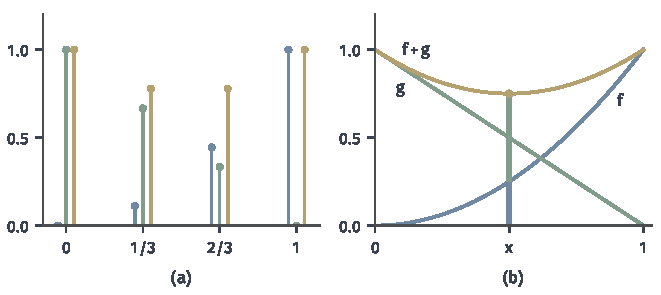
\includegraphics[width=112mm]{figures/04-spaces-measures-and-geometry/03-function-spaces/matplotlib/fvec-pointwise-addition/figure.pdf}
  \caption{函数相加就是逐分量相加。蓝色为$f(x)=x^2$，绿色为$g(x)=1-x$，黄色为二者之和。(a)四个采样点上的取值，每点从左到右依次是$f$、$g$、$f+g$的分量。(b)全部输入上的曲线；在一个固定的$x$处，蓝色线段与绿色线段接起来的总高度等于$f(x)+g(x)$。}
  \label{fig:fvec-pointwise-addition}
\end{BookInlineFigure}

现在写出一般的定义。固定一个非空集合$X$，称为输入集合，考虑全体函数$f:X\to\mathbb K$组成的集合，记为$\mathbb K^X$。这个记号本身就是类比：$\mathbb K^d$的元素给每个下标$k\in\{1,\ldots,d\}$指定一个数，$\mathbb K^X$的元素给每个$x\in X$指定一个数。两个函数的和与一个函数的数乘都在每个输入处分别计算：
\begin{equation}
 (f+g)(x)=f(x)+g(x),\qquad (cf)(x)=c\,f(x),
 \label{eq:fvec-pointwise-operations}
\end{equation}
其中$x\in X$，$c\in\mathbb K$。零元素是处处取零的\term{零函数}（zero function），$f$的负元是$x\mapsto-f(x)$。式~\eqref{eq:fvec-pointwise-operations}称为\term{逐点运算}（pointwise operations）。

逐点运算满足线性空间的八条运算规则，验证方法是把每条规则放到一个固定的输入处检查。以加法交换律为例，要证$f+g=g+f$，而两个函数相等的意思是它们在每个输入处取值相同。任取$x\in X$，由式~\eqref{eq:fvec-pointwise-operations}和数的交换律，
\[
 (f+g)(x)=f(x)+g(x)=g(x)+f(x)=(g+f)(x).
\]

结合律、分配律和零元、负元的规则都这样逐点继承自$\mathbb K$中的运算，所以$\mathbb K^X$在逐点运算下是$\mathbb K$上的线性空间。这与验证$\mathbb K^d$是线性空间时逐分量检查的做法相同。线性空间与子空间的一般定义、基与坐标，可参考\BookChapterRef{chap:linear-representation}{卷二第2章“线性空间、映射与坐标”}。

改变输入集合$X$，就得到熟悉的对象。取$X=\{1,\ldots,d\}$，函数就是$d$维向量。取$X=\mathbb N_+=\{1,2,3,\ldots\}$，一个函数$x:\mathbb N_+\to\mathbb K$就是一个数列$x=(x_1,x_2,\ldots)$，其中$x_k=x(k)$，式~\eqref{eq:fvec-pointwise-operations}这时是逐项相加与逐项数乘。取$X=[0,1]$，就是区间上的函数。图~\ref{fig:fvec-index-to-function}把这三种情形放在一起：横轴都是“下标”，纵轴都是“这个下标上的数”。

\begin{BookInlineFigure}
  \centering
  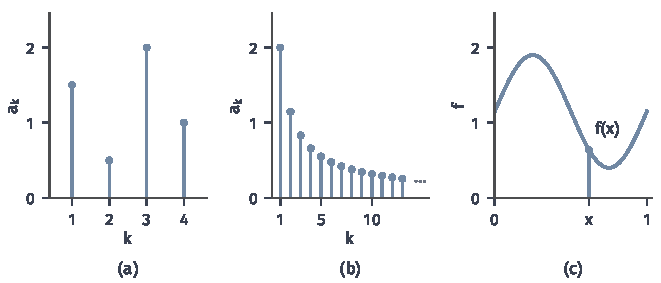
\includegraphics[width=112mm]{figures/04-spaces-measures-and-geometry/03-function-spaces/matplotlib/fvec-index-to-function/figure.pdf}
  \caption{同一种构造的三个例子。(a)$X=\{1,2,3,4\}$时是四维向量。(b)$X=\mathbb N_+$时是数列，下标可以一直延伸下去。(c)$X=[0,1]$时下标连成一片，竖线所示的是下标$x$上的数$f(x)$，竖线的顶点连成了函数的图像。}
  \label{fig:fvec-index-to-function}
\end{BookInlineFigure}

类比在这里出现第一个边界。$X=[0,1]$时，输入有不可数个，无法排成$a_1,a_2,\ldots$这样的一列，所以$[\ldots,f(x),\ldots]$只是一幅图景，不是真的列表。好在式~\eqref{eq:fvec-pointwise-operations}用不着排序，它只要求对每个$x$分别计算。表~\ref{tab:fvec-dictionary}汇总了目前的对应关系。

\begin{BookInlineTable}
  \centering
  \begin{tabular}{@{}ll@{}}
    \toprule
    有限维向量$a\in\mathbb K^d$ & 函数$f\in\mathbb K^X$\\
    \midrule
    下标$k\in\{1,\ldots,d\}$ & 输入$x\in X$\\
    分量$a_k$ & 取值$f(x)$\\
    逐分量相加$a+b$ & 逐点相加$f+g$\\
    逐分量数乘$ca$ & 逐点数乘$cf$\\
    零向量 & 零函数\\
    $a=b$：每个分量相等 & $f=g$：每个输入处取值相等\\
    \bottomrule
  \end{tabular}
  \caption{有限维向量与函数的对应。左右两列的运算规则相同，差别只在下标集合。}
  \label{tab:fvec-dictionary}
\end{BookInlineTable}

\paragraph{线性子空间的核验}
实际使用的通常不是全体函数，而是满足某种要求的函数，例如连续函数或多项式。这就像在$\mathbb R^3$中只看一个过原点的平面。要在这样的集合$V\subseteq\mathbb K^X$中继续使用线性空间的语言，须核对三条：零函数属于$V$；$V$中两个函数之和仍在$V$中；$V$中函数的数乘仍在$V$中。三条都成立时，$V$是$\mathbb K^X$的线性子空间，本身也是线性空间，下面简称为\term{函数空间}（function space）。

几个常用的集合都通过了核验。闭区间上的连续函数全体$C[a,b]$是线性子空间，因为常数零连续，连续函数的和与数乘仍连续。次数不超过$m$的多项式全体$P_m$是线性子空间，因为两个这样的多项式相加不会提高次数。

数列也有同样的例子。收敛到零的数列全体记为$c_0$，它是线性子空间：若$x_k\to0$、$y_k\to0$，则$x_k+y_k\to0$，$cx_k\to0$。只有有限项非零的数列全体记为$c_{00}$，它也是线性子空间，因为两个数列的非零项都只有有限个时，和的非零项也只有有限个。

约束一个分量的取值，能看出子空间与非子空间的区别。集合$\{f\in C[0,1]:f(0)=0\}$把“下标$0$上的分量”固定为零，它是线性子空间，正如$\mathbb R^3$中的平面$x_1=0$。集合$\{f\in C[0,1]:f(0)=1\}$则对应不过原点的平面$x_1=1$：它不含零函数，两个成员相加后在$0$处取$2$，也不封闭。

失败还可以更隐蔽。$\mathbb R^2$中两条坐标轴的并集对数乘封闭，但$(1,0)+(0,1)$已经离开了这个集合。函数空间中也有同样的情形，考虑参数族
\[
 \mathcal R=\{x\mapsto a\max(0,x-t):a,t\in\mathbb R\},
\]
其中每个成员的图像是一条折线，斜率至多改变一次。

取$\mathcal R$中的两个成员$f(x)=\max(0,x)$与$g(x)=\max(0,x-1)$，分段写出它们的和：
\[
 (f+g)(x)=\begin{cases}0,&x\leq0,\\x,&0<x\leq1,\\2x-1,&x>1.\end{cases}
\]
斜率在$x=0$处由$0$变为$1$，在$x=1$处由$1$变为$2$，共改变两次，所以$f+g\notin\mathcal R$。$\mathcal R$对数乘封闭、对加法不封闭，和两条坐标轴的并集属于同一类。这样的族可以作为逼近工具，但不能直接当作线性空间使用。

\paragraph{函数值、函数元素与坐标}
向量有下标$k$、分量$a_k$和整个向量$a$三个层次，函数也一样。输入$x\in X$是一个位置；$f(x)\in\mathbb K$是这个位置上的数；$f$本身是整条对应规则，是函数空间中的一个元素。说“$f=g$”是在比较元素，要求所有位置的值都相同；说“$f(x_0)=g(x_0)$”只比较了一个位置。

坐标是另一回事，它依赖另外选定的基。在$P_2$中取多项式$p(x)=2-x+3x^2$，相对于基$1,x,x^2$，它的坐标是系数$(2,-1,3)$。改用基$1,x-1,(x-1)^2$时，要把$p$按$x-1$重新整理。令$t=x-1$，把$x=t+1$代入$p$，得到
\[
 p=2-(t+1)+3(t+1)^2.
\]
展开平方并合并同类项，得到
\[
 p=4+5t+3t^2.
\]
换回$x$，就是
\[
 p(x)=4+5(x-1)+3(x-1)^2,
\]
所以新的坐标是$(4,5,3)$。

元素$p$没有变，变的是记录它的方式。这与卷二中同一个向量在两组基下有两列坐标是一回事。图~\ref{fig:fvec-two-coordinates}中两张图的蓝色曲线是同一条，只是拆成了不同的三个部分。

\begin{BookInlineFigure}
  \centering
  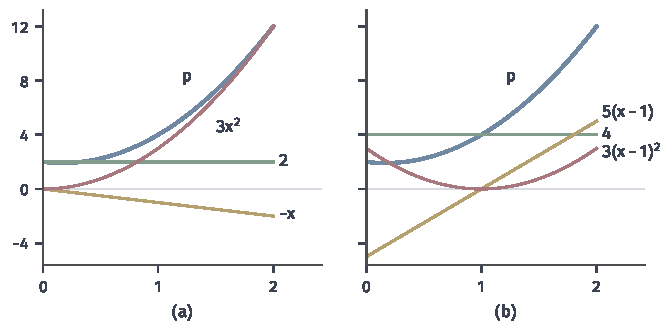
\includegraphics[width=112mm]{figures/04-spaces-measures-and-geometry/03-function-spaces/matplotlib/fvec-two-coordinates/figure.pdf}
  \caption{同一个函数的两种分解。蓝色曲线都是$p(x)=2-x+3x^2$。(a)拆成$2$、$-x$、$3x^2$三部分，坐标为$(2,-1,3)$。(b)拆成$4$、$5(x-1)$、$3(x-1)^2$三部分，坐标为$(4,5,3)$。在每个$x$处，同一张图中三条细线的高度之和等于蓝色曲线的高度。}
  \label{fig:fvec-two-coordinates}
\end{BookInlineFigure}

函数值$p(1)=4$恰好等于第二组坐标的第一项，因为另外两个基函数在$x=1$处都为零。这是这组基的性质，不是坐标的一般含义：第一组坐标的第一项$2$等于$p(0)$，并不等于$p(1)$。

至此，一个函数有了两种“一列数”。一种是取值列，下标是输入$x$，它不需要选基。另一种是系数列，下标是基函数的编号，它随基改变。本章开头的$[\ldots,a_1,a_2,\ldots]$可以按这两种方式来读，下一节会把二者的关系写成矩阵。

\paragraph{乘法与微分不是一般的内部运算}
向量也可以逐分量相乘，但线性空间的定义用不到这种运算。函数同样如此：逐点乘法$(fg)(x)=f(x)g(x)$在某些集合上有意义，却不属于线性结构。$P_m$对乘法不封闭，因为$x^m\in P_m$，而$x^m\cdot x=x^{m+1}\notin P_m$。

求导$f\mapsto f'$也要看空间。$C[0,1]$对乘法封闭，对求导却不封闭：$f(x)=\lvert x-\tfrac12\rvert$连续，但在$\tfrac12$处不可导，$f'$不是$[0,1]$上处处有定义的函数。

所以讨论某个函数空间时，加法与数乘是自带的运算；乘积和导数是另外的操作，要单独说明它们从哪个空间送到哪个空间。例如求导把$P_2$送入$P_2$，而且是线性的。若用基$1,x,x^2$的坐标表示，把$a_0+a_1x+a_2x^2$求导得到$a_1+2a_2x$，这个操作就是一个矩阵：
\[
 \begin{bmatrix}a_1\\2a_2\\0\end{bmatrix}
 =\begin{bmatrix}0&1&0\\0&0&2\\0&0&0\end{bmatrix}
 \begin{bmatrix}a_0\\a_1\\a_2\end{bmatrix}.
\]

把前面的$(2,-1,3)$代入，得到$(-1,6,0)$，也就是$p'(x)=-1+6x$。乘一个固定函数$g$的操作也有这样的矩阵形式：在采样点上，它是对角元为$g(x_1),\ldots,g(x_n)$的对角矩阵。这样的映射在无限维空间中称为线性算子，在第~\ref{chap:linear-operators}章研究；可微性的推广则由第~\ref{chap:smoothing-weak-derivatives}章的弱导数承担。
